\chapter{Methodological notes}\label{chap:method}

In this chapter I present, somewhat informally, the statistical and data visualization tools I will use in the rest of this book. Readers interested in the mathematical details should consult the cited sources, since detailed descriptions and explanations of these techniques would merit a short book and a strong statistical background. My intention is only to provide the reader with a good intuition of what these methods do.

\section{On the general methodology}

Many of the phenomena I discuss in the following case studies have been studied exhaustively before, and it is not my intention to develop complete analyses for any of these cases. Moreover, in several instances, I will use sub-optimal models that ignore semantics or other possible strong predictors, this should only make the main point stronger: formal analogy occurs even in unexpected cases, and it follows the grammatical hierarchy of the language. Similarly, I do not provide full formal linguistic analyses, but rather only sketches to motivate a plausible type hierarchy. It is my intention that  the ideas proposed in this book can be formally implemented in different linguistic theories (Construction Grammar, Cognitive Grammar, Paradigm Function Morphology, \textsc{hpsg} or similar). This is why theoretical assumptions are kept to a minimum.

I make no strong claims concerning the psycho-linguistic reality to these models. The fact that we can predict, to a greater or lesser degree, word classes from formal properties of words, does not mean that speakers necessarily do the same. It is possible that the way speakers perform class assignment in some of the languages studied has some parallels to the models proposed here, but it is also possible that speakers do rely on different aspects of cognition. These are related but independent questions. The patterns I will present could be productive, or vestiges of previous systems, but not any less real. I will, however, make some connections with some ideas about cognitive aspects of language during the final discussion.

There are t two main reasons for the choice of languages in this study: theoretical relevance and data availability. I have not tried to compile a  representative typological sample. Far from it, most examples are from Indo-European languages of various subfamilies, and only a few are taken from African languages. The analogical models require an electronic, morphologically annotated dictionary, which are still very rare for languages spoken by smaller language communities. The theoretical relevance relates to the classes a language has and how they are organized.

\section{Statistical models and methodology}

For all the cases to follow I use the same general method for building the analogical models. From the stem of the words (nouns or verbs) I extract predictors which might be at play in the analogical relations and fit a neural network with the \texttt{nnet} package \autocite{Venables.2002}\footnote{For all models I used the \texttt{softmax} linking function and the maximum number of weights and iterations set in a way that the models converge. Whether a hidden layer was present or not, and the number of hidden units, varied from model to model.} in R \autocite{RDevelopmentCoreTeam.2008}. The use of neural networks has a long history in linguistics, and they are usually linked to connectionist models \autocite{Bechtel.2002, Churchland.1989, McClelland.1986, Rumelhart.1986}. However, I do not make any claims about the underlying linguistic system, or the rightness or wrongness of connectionism. The use of neural networks for the following analogical models is purely practical. Similar effects could probably be achieved using different algorithms like Random Forest \autocite{Breiman.2001a} or Support Vector Machines \autocites{Smola.1998, Scholkopf.2001}. For the present book, the actual technology is not important, only the concept behind it\footnote{The next subsection provides a simple illustration of how the analogical models work, but the interested reader should consult \textcite{Venables.2002} for a rigorous mathematical explanation of neural networks and the \texttt{nnet} package.}. My aim is to show that prediction is possible, not to find the best possible method.

The \textit{stems} in the models are not theoretical objects, and the ideas in these models should be compatible with word-based models. The idea is that there is a distinction between the phonological material that expresses some property like \textsc{masculine}, and the phonological material that expresses the meaning `cat'. I take the \textit{stem} to be the full word minus the phonological material that marks the category at hand. In a trivial Spanish example, the stem of \textit{gato} (`male cat') is \textit{/gat/}, since the \textit{/o/} segment is the gender correlate, and we have the opposing form \textit{gata} (`female cat'). For many non-trivial cases some compromise had to be reached, and it will be described in detail. Crucially, this approach does not consider underlying representations, only surface forms. Of course, one could compare the results of a model based on some sort of underlying representation with the results of more surface oriented models.

The predictors used to fit the analogical models vary slightly from model to model, but they always contain phonological information about the shape of the word. The most straightforward way to do this is to simply take a set number of letters at the end (or beginning) of the stems and use them (together with their position) as predictors. What the positional information does is to make a distinction between, say, a \textit{t} at the end of the stem and a \textit{t} in the third to last position. This way of specifying phonological shape has advantages and disadvantages. A good aspect of this approach is that the model can, on its own, infer classes between phonemes as represented by letters. If \textit{x} and \textit{h} share some phonological feature which makes them into a natural class, and are thus predictive of the same inflection class or gender, the model will simply assign the corresponding weights to said inflection class. This means that we do not need a rich phonological representation to arrive at phonological analogies. Another possible issue, which might unfairly benefit or harm the models, is that in cases of low correspondence between the phonology and the orthography, certain spelling rules might contain some additional information not directly available to speakers, or some important information might be missing. There is no easy way to solve this problem, short of using detailed phonological transcriptions, which are unavailable for most of the languages under consideration. Any sort of phonological process like methathesis, which could be easily captured by a rule-based approach, will be invisible to the model, thus reducing the amount of information available. To reduce loss of information due to some spelling systems representing a single phoneme with a character sequence (e.g. Spanish and German), I simplified spelling assigning special characters to those regular sequences. Some phonological information is, however, non-recoverable from the orthography (e.g. some vowel length/quality information in German, or the difference between long and double vowels in Kasem).

To prevent overfitting\footnote{Overfitting happens when models predict the same items they learned from. This is a problem because if a model is overfitted, it does not really tell us much about how good the predictors are on novel items.} the models I apply ten-fold cross-validation to every model. This is done by splitting the dataset into ten groups. The general model is then fitted using nine of the groups as training data and testing the predictions of the model on the group not used for fitting it. The process is repeated for each of the ten subgroups. This way we can look at all the data while preventing  overfitting \autocite{Kohavi.1995}.

In section \sectref{sec:mechanisms-analogy} I discussed four possible ways of implementing analogy, and argued that the difference is a gradient rather than a truly categorical one. The present models fall somewhere between a weighted multiple-rule-based model like those presented by \textcite{Albright.2003} and \textcite{Albright.2009} and a purely stochastic model like NDL \autocites{Arppe.2014, Baayen.2011, Baayen.2011a} or AM \autocites{Skousen.1989, Skousen.2002, Skousen.2013, Arndt-Lappe.2011, Arndt-Lappe.2014}. The difference between the present model and a weighted rule-based model is that I consider all possible patterns within some structurally defined positions in the word (e.g. the last two segments, the last consonant, the number of syllables, etc.), and do not attempt to predefine the rules of the model, or decide to include or exclude some patterns. The difference to a completely stochastic system lies in the same property: the current model is sensitive to structural properties of the lexemes it sees, while NDL and AM are ``blind'' or completely amorphous. Like AM, and unlike some previous connectionist systems \autocite{Bechtel.2002, Churchland.1989, McClelland.1986, Rumelhart.1986}, the analogical model used here sees linguistically defined categories as the outputs. In traditional connectionist systems the networks directly paired semantics to sounds \autocite{Matthews.2005}.

The similarities between these kinds of systems have been observed before:

\begin{quotation}
Connectionist  networks  themselves  further  illustrate  the  problem,  in  that  they might be seen to fall in both camps. Back-propagation networks are often described as  depending  on  similarity\dots  However,  they  are  also often described as using ‘implicit rules’ which can be extracted using appropriate analysis\dots Therefore, back-propagation networks appear rule- and similarity-based \autocite[p. 200]{Hahn.1998}
\end{quotation}

In any case, it should be clear that I am not arguing for neural networks as a necessarily better implementation of analogical systems, or as a psychologically plausible system. Neural networks as used here are just one of the many alternatives we have to model analogy.

All this being said, a more clever and carefully designed model similar to the weighted multiple-rule-based model like those presented by \textcite{Albright.2003} and \textcite{Albright.2009}, or that of \textcite{Beniamine.2016}, would probably perform better for any particular case and be more psychologically plausible. These models have some downsides, however. The most important one is that they require much better structured datasets, with complete phonological information. This requirement is harder to fulfill than the rough, semi-phonemic transcriptions required for the neural network models. A second difficulty of these models is that they are extremely slow to fit because the rule inference step is computationally intensive. This makes it impossible in practice to fit many different models for each case and hence impractical to test various combinations of predictors.

\section{Analogical models using neural networks}

The easiest way to explain the intuition behind the models, and the tools I use for evaluating them, is with concrete examples. Suppose a language has two inflection classes, \textbf{A} and \textbf{B}. The dataset in \REF{exe-inflect-1} presents stems for lexemes belonging two said inflection classes.

\begin{exe}
    \ex  \label{exe-inflect-1}
    \begin{xlist}
        \ex A: \textit{lama}, \textit{lara}, \textit{lado}, \textit{laso}, \textit{pama}, \textit{ra}, \textit{dal}, \textit{kar}, \textit{tsar}, \textit{sek}, \textit{cess}
        \ex B: \textit{egrr}, \textit{liz}, \textit{lo}, \textit{loi}, \textit{lu}, \textit{lip}, \textit{roop}, \textit{oppe}, \textit{toi}, \textit{olor}, \textit{gin}, \textit{grip}, \textit{wik}
    \end{xlist}
\end{exe}

There is no single (simple) rule which can predict to what class a given lexical item belongs. However, intuitively, the first vowel seems to be a strong indicator. All items for which the first vowel is \textit{a} belong to class A, while items for which the first vowel is \textit{i}, \textit{o} or \textit{u} belong to class B. Items with \textit{e} are found in both groups. Because there are only a few lexical items, and the pattern is fairly simple, this generalization is fairly evident, but in a more complex system it would be much harder. These observations could also be inferred with a statistical model.

Put in simple terms, given a training dataset with items, and a series of predictors for each item, the neural network model learns from these items and assigns weights to the predictors. When presented with new data (the testing dataset), the network calculates from the weights the probability of each outcome for each item in the dataset. This is achieved the following way. The neural network sets a baseline for the prediction, based on one of the levels for each predictor. For each predictor, the first level (alphabetically) is chosen for the baseline node (in this case thus: \texttt{s1}=\textit{c}, \texttt{s2}=\textit{a}). This baseline has a weight for each outcome (the classes to be predicted). To each other level of each predictor, it assigns a weight for each outcome. The weights of the predictors are added to the baseline to calculate the probability of each outcome given some input.

We can apply this to our previous example. We split the data set into a training and a small testing dataset. For the testing dataset we randomly select the items: \textit{lama}, \textit{lara}, \textit{kar}, \textit{egrr}, \textit{liz}, \textit{oppe}, \textit{grip}, and we assign the rest of the items to the training dataset. For illustration, we can fit two different models. In Model 1, we set two predictors \texttt{s1} and \texttt{s2}, which correspond to the first and second letter in the items, respectively. For Model 2 we set \texttt{v1} and \texttt{c1}, which correspond to the first vowel and first consonant of the items, respectively. We can then train Model 1 and Model 2.

\figref{fig:model1} shows the structure of the neural network for Model 1. As can be seen, there is a direct connection between the predictors and the outcomes (a skip layer), and there are no intermediate steps (hidden layers). We can see how each letter predicts A or B. The thickness of the line represents the absolute value of the weight (thicker lines have larger absolute values), and the color represents whether the weight is positive (dark gray) and favors the outcome, or negative (light gray) and disfavours the outcome. In the node marked as \texttt{B1} we have the baseline (the bias node) made up of the combination of the levels \textit{c} for \texttt{s1} and \textit{a} for \texttt{s2}\footnote{The models chooses the baseline levels purely on alphabetical order.}. This combination clearly favours \textbf{A}, as we would expect. If any of these levels changes in the input, then the nodes in the skip layer activate and counteract the baseline. If, say, the input contains an \textit{u}, \textit{i} or \textit{o} instead of an \textit{a} in \texttt{s2}, then the corresponding node will strongly activate the outcome \textbf{B}, as we, again, would expect from the data set. The complete set of weights from the inputs to the outcomes for Model 1 is given in \tabref{tab:model1-weights}.

\begin{sidewaysfigure}[!htpb]
  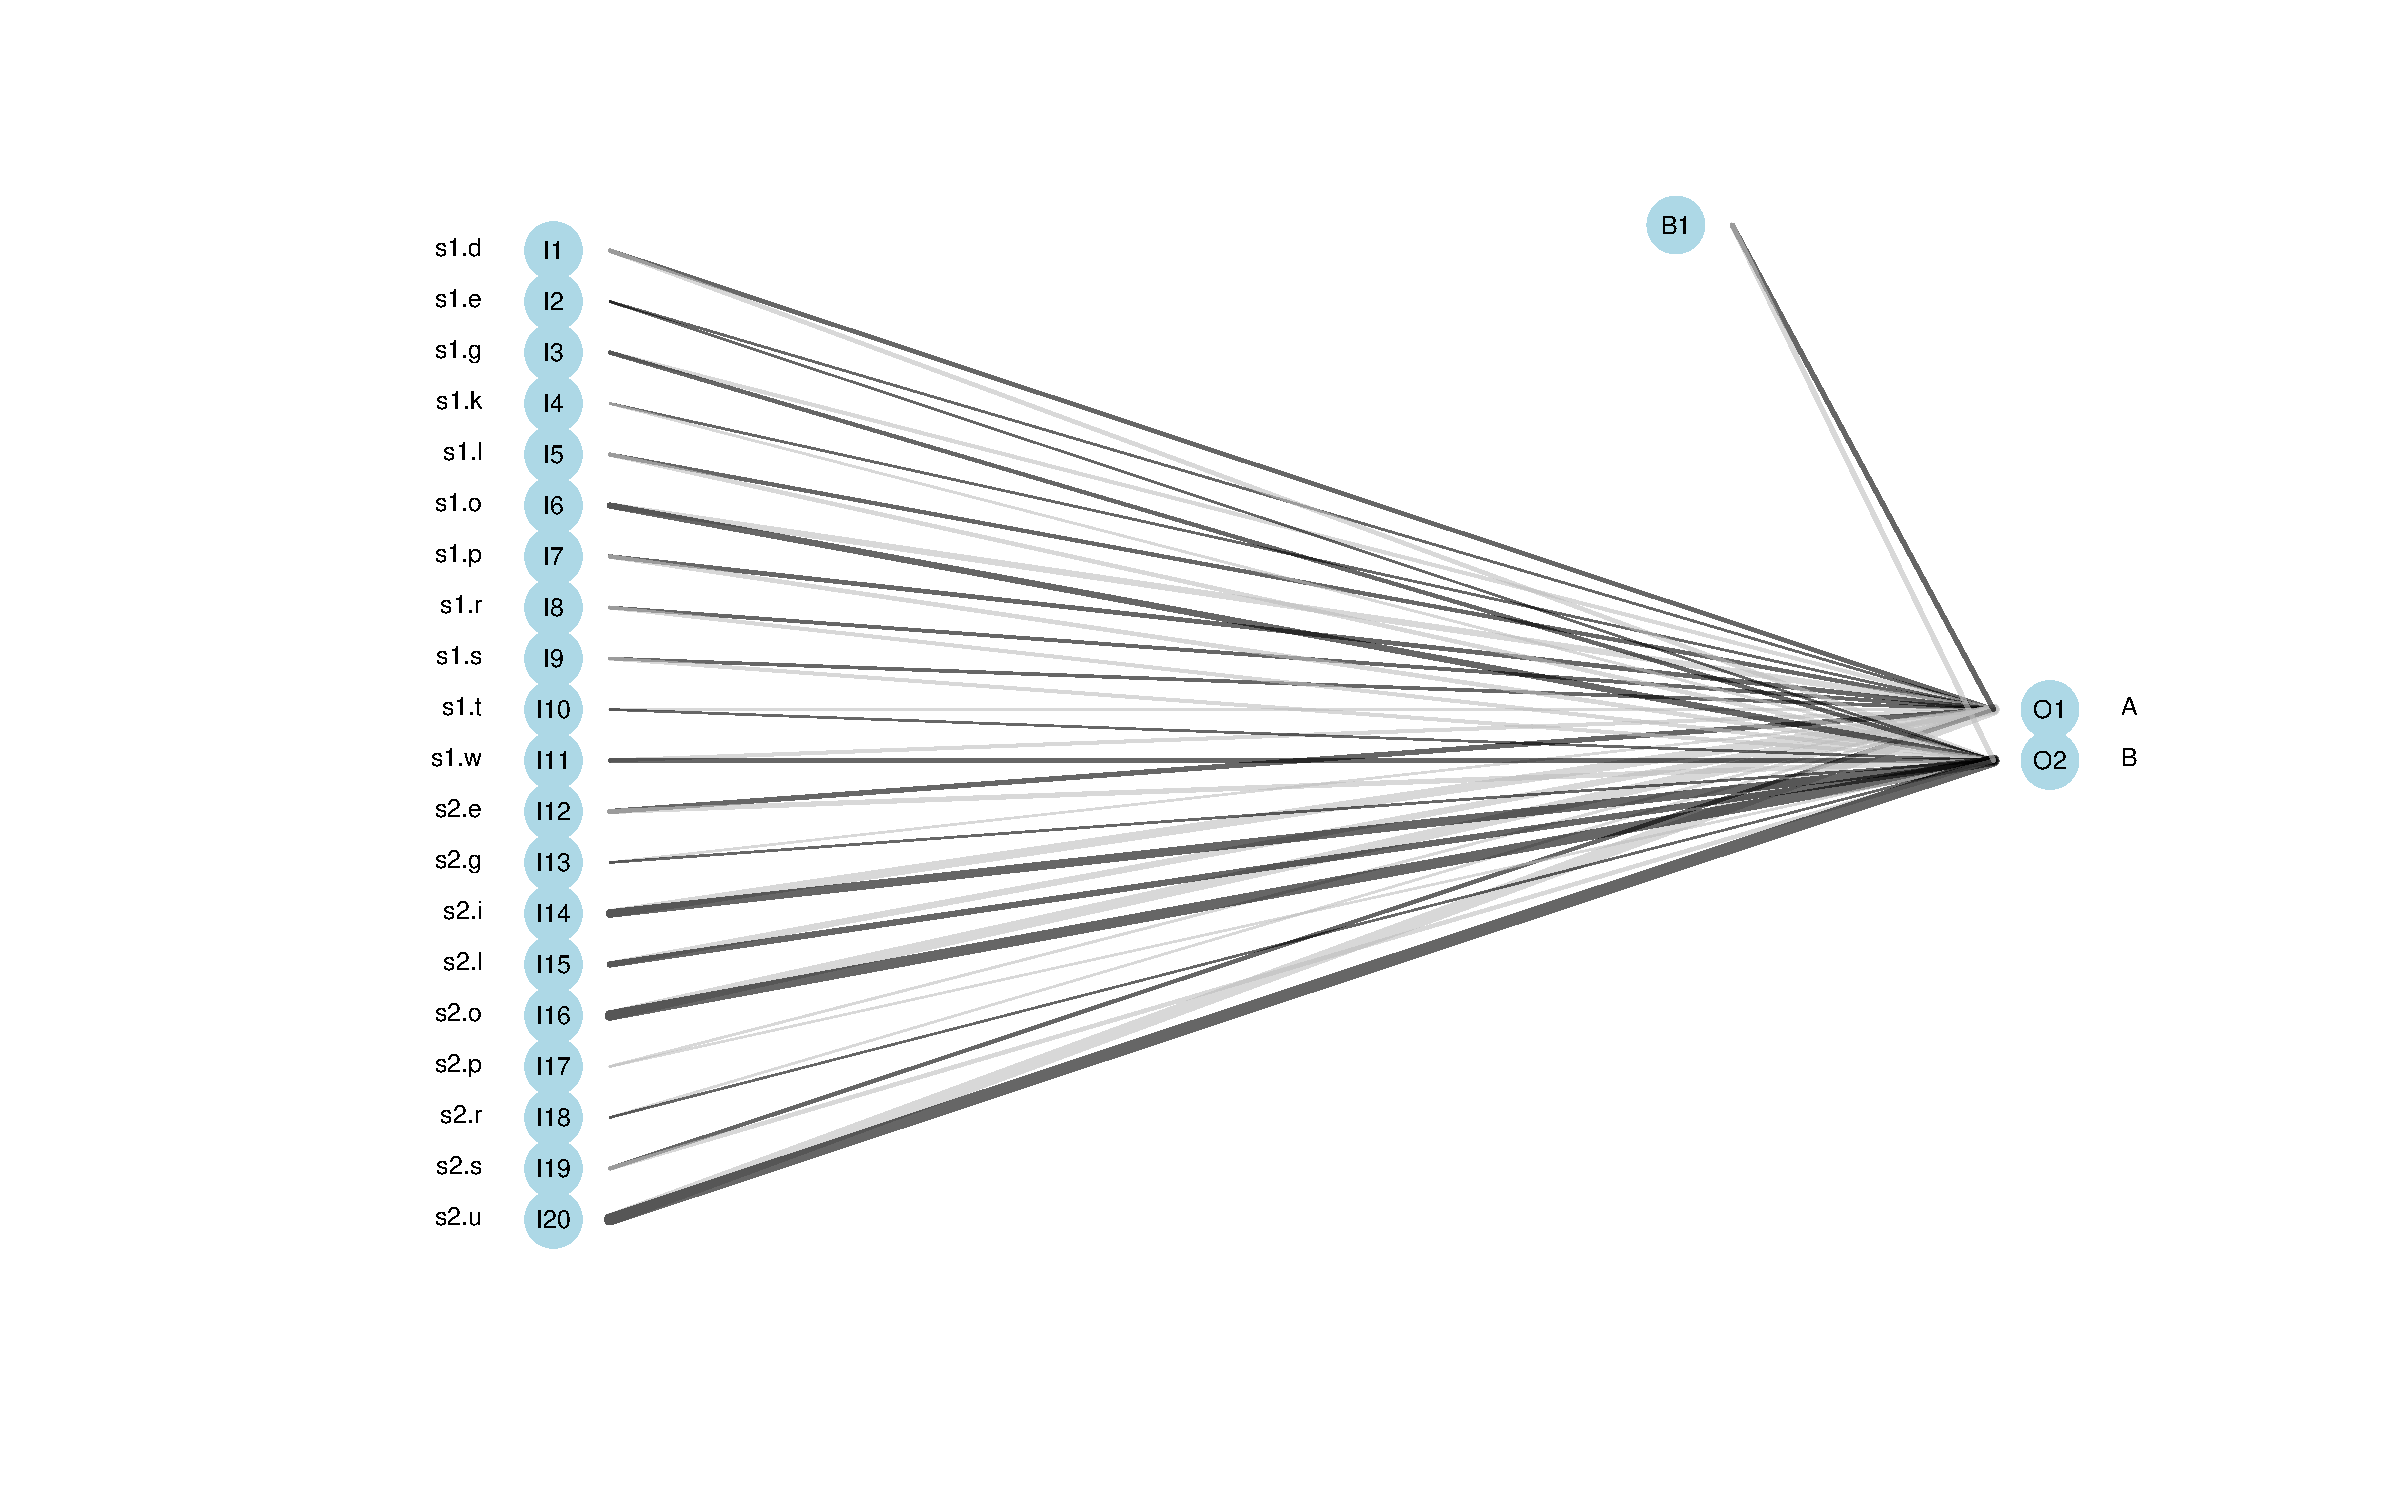
\includegraphics[scale=0.45]{./figures/fake/model1.pdf}
  \caption{Representation of Model 1.}\label{fig:model1}
\end{sidewaysfigure}

\begin{table}[!htpb]
    \centering
    \small
\renewcommand{\arraystretch}{0.90}% Tighter
  \begin{tabular}{lllll}
    \lsptoprule
       & weight & predictor & response & variable \\
    \midrule
    1  & 5.42   & c-a       & A        & baseline \\
    2  & 3.43   & d         & A        & s1       \\
    3  & -0.29  & e         & A        & s1       \\
    4  & -3.21  & g         & A        & s1       \\
    5  & 0.58   & k         & A        & s1       \\
    6  & 2.89   & l         & A        & s1       \\
    7  & -7.13  & o         & A        & s1       \\
    8  & 4.37   & p         & A        & s1       \\
    9  & 1.89   & r         & A        & s1       \\
    10 & 2.24   & s         & A        & s1       \\
    11 & 0.81   & t         & A        & s1       \\
    12 & -2.62  & w         & A        & s1       \\
    13 & 4.67   & e         & A        & s1       \\
    14 & 0.61   & g         & A        & s1       \\
    15 & -13.22 & i         & A        & s1       \\
    16 & -8.12  & l         & A        & s1       \\
    17 & -14.45 & o         & A        & s1       \\
    18 & 0.03   & p         & A        & s1       \\
    19 & -0.33  & r         & A        & s1       \\
    20 & 4.25   & s         & A        & s1       \\
    21 & -18.31 & u         & A        & s1       \\
    22 & -5.43  & c-a       & B        & baseline \\
    23 & -3.88  & d         & B        & s2       \\
    24 & -0.35  & e         & B        & s2       \\
    25 & 3.28   & g         & B        & s2       \\
    26 & 0.49   & k         & B        & s2       \\
    27 & -2.19  & l         & B        & s2       \\
    28 & 7.49   & o         & B        & s2       \\
    29 & -4.96  & p         & B        & s2       \\
    30 & -2.67  & r         & B        & s2       \\
    31 & -2.02  & s         & B        & s2       \\
    32 & -0.49  & t         & B        & s2       \\
    33 & 2.95   & w         & B        & s2       \\
    34 & -5.20  & e         & B        & s2       \\
    35 & -0.48  & g         & B        & s2       \\
    36 & 12.77  & i         & B        & s2       \\
    37 & 8.35   & l         & B        & s2       \\
    38 & 13.70  & o         & B        & s2       \\
    39 & -0.38  & p         & B        & s2       \\
    40 & -0.11  & r         & B        & s2       \\
    41 & -3.81  & s         & B        & s2       \\
    42 & 17.85  & u         & B        & s2       \\
    \lspbottomrule
  \end{tabular}\caption{Weight table for Model 1.}\label{tab:model1-weights}
\end{table}

To calculate the actual class probabilities from the output weights, we use the softmax function. The intuition of this function is that, given a vector of weights, it will transform that vector into a vector of probabilities, where the element with the highest weight will receive the highest probability, and all probabilities add up to 1. The general form of this function is given in equation \eqref{eq:softmax}. In prose, we exponentiate each weight, and divide by the sum of all exponentiated weights.  

\is{Softmax}

\begin{equation}\label{eq:softmax}
    S(y_i) = \frac{e^{y_i}}{\sum_{j}^{e^{y_j}}}
\end{equation}

As an example, assume the weight vector [2, 1, 0.1]. Exponentiating each member we get the vector [7.4, 2.7, 1.1], and their sum is 11.21. Dividing the exponentiated weights by the sum we get the probabilities [0.66, 0.24, 0.1].

To know how well the model performs, we predict the outcomes of the testing dataset, build a confusion matrix and calculate different accuracy scores. The corresponding confusion matrix for this model is shown in \tabref{tab:model1-conf}. Here we see the predictions that the model made for each testing item. There were two errors in total: \textit{egrr} and \textit{grip}. It is easy to see why these errors happen: there are no comparable items in the training dataset, \textit{grip} starts with a \textit{gr} sequence and \textit{egrr} is the only item with an \textit{e} as first letter and \textit{g} as second letter.

\tabref{tab:model1-conf} shows the confusion matrix for the predictions of Model 1, and \tabref{tab:tpfp-conf} shows a matrix with the positions of True Positives (TP), True Negatives (TN), False Positives (FP) and False Negatives (FN). The TP and TN are cases where the class predicted by the model match the real class of the items. FP and FN are the cases where the class predicted by the model does not match the real class of the items. The total population \textit{N} is the sum of all these values: $\textrm{TP}+\textrm{TN}+\textrm{FP}+\textrm{FN}$.

\begin{table}[!htpb]
  \centering
  \begin{tabular}{llll}
    \lsptoprule
    & Predicted & Observed & Word \\
    \midrule
    1 & A & A & lama \\
    2 & A & A & lara \\
    3 & A & A & kar \\
    4 & A & B & egrr \\
    5 & B & B & liz \\
    6 & B & B & oppe \\
    7 & A & B & grip \\
    \lspbottomrule
  \end{tabular}
  \caption{Predictions Model 1.}\label{tab:preds-model1}
\end{table}

\begin{table}[!htpb]
  \centering
  \begin{tabular}{rrrr}
    \lsptoprule
               & \multicolumn{3}{c}{Reference} \\
    \midrule
    Prediction & A  & B                        \\
    A          & 3  & 2                        \\
    B          & 0  & 2                        \\
    \lspbottomrule
  \end{tabular}
    \caption{Confusion matrix for Model 1.}\label{tab:model1-conf}
\end{table}

\begin{table}[!htpb]
  \centering
  \begin{tabular}{rrrr}
    \lsptoprule
               & \multicolumn{3}{c}{Reference} \\
    \midrule
    Prediction & A  & B                        \\
    A          & TP & FP                       \\
    B          & FN & TN                       \\
    \lspbottomrule
  \end{tabular}
  \caption{Diagram of True Positives, False Positives, True Negatives and False Negatives.}\label{tab:tpfp-conf}
\end{table}

The accuracy is the number of correct predictions divided by the total number of items. Additionally, we can calculate the confidence interval (CI) of the accuracy by using a binomial test \autocite{Clopper.1934, Newcombe.1998}. The No Information Rate (or accuracy of a model under a no information situation) is calculated as the largest class percentage in the data. In this case, \textbf{A}'s class percentage is 0.4286 and \textbf{B}'s is 0.5714, thus the latter is taken to be the No Information Rate. In other words, the No Information Rate is the accuracy of a model that always predicts the most frequent outcome. In our example data \textbf{B} is the most frequent outcome. If the model predicted all outcomes to be \textbf{B}, then it would reach an accuracy of $4/7=0.5714$. Models where all predictors have no information regarding the outcomes (i.e. they are poor predictors) tend to have an accuracy close to the No Information Rate, because always predicting the most frequent outcome guarantees the highest possible accuracy under a no information situation. The model is then said to perform above chance if the No Information Rate is less than the lower limit of the accuracy confidence interval.

There are three additional statistical values I will use in certain cases are: \textit{Specificity}, \textit{Sensitivity} and \textit{Negative Predictive Value}. Specificity is the proportion of negatives that are identified as such ($=\textrm{TN}/(\textrm{TN}+\textrm{FP})$), while sensitivity is the proportion of positives that are identified as such ($=\textrm{TP}/(\textrm{TP}+\textrm{FN})$). The negative predictive value ($=\textrm{TN}/(\textrm{TN}+\textrm{FN})$) will help us identify the class to which more items from other class are misclassified. These three statistics are not relevant for this particular example because we only have two classes here, but can be used, by class, in models with more than two outcomes.

Finally, the kappa statistic compares the observed accuracy with the expected accuracy (under random chance). The expected accuracy is calculated as follows. We multiply the observed frequency of \textbf{A} by the predicted frequency of \textbf{A}, and the observed frequency of \textbf{B} by the predicted frequency of \textbf{B}. We then divide these numbers by N, add them together and divide again by N. Thus, we get:

\is{True Positive}
\is{True Negative}
\is{False Positive}
\is{False Negative}
\is{Expected Accuracy}

\begin{equation}
    \textrm{Expected.Accuracy}=\frac{\frac{(\textrm{TP}+\textrm{FN})*(\textrm{TP}+\textrm{FP})}{\textrm{N}} + \frac{(\textrm{TN}+\textrm{FP})*(\textrm{TN}+\textrm{FN})}{\textrm{N}}}{\textrm{N}}
\end{equation}

Finally to calculate the kappa statistic we use the following equation:

\begin{equation}
  \textrm{Kappa} = \frac{\textrm{observed.accuracy} - \textrm{expected.accuracy}}{1 - \textrm{expected.accuracy}}
\end{equation}

\is{Kappa score}
\is{Accuracy}

Kappa scores\footnote{In our case: $\textrm{Expected.Accuracy}=\frac{\frac{3*(3+2)}{7} + \frac{2*(2+2)}{7}}{7} = \frac{\frac{15}{7}+\frac{4}{7}}{7} = 0.4694$. The accuracy is $5/7=0.7143$. Thus, we have that $\textrm{kappa} = \frac{0.7143 - 0.4694}{1 - 0.4694}=0.4615$. Notice that the Expected Accuracy is different from the No Information Rate because the former is taken from a model that knows about the distribution of the outcomes in the traning dataset, while the latter is a completely random assignment of outcomes to inputs in the testing dataset.} go from 0 (in a perfectly random model) to 1 (in a perfectly accurate model), a kappa of 0.5 is halfway between the expected accuracy and 1. The advantage of using kappa is that it tells us how well above random chance the model is performing, and, to a degree, it allows to make model comparisons. The disadvantage is that there is no standarized interpretation and no objective cutoff point. A model with a kappa of 0.2 is not inherently bad, nor can it be said that it is at chance level. However, we can say that a model with a kappa of 0.7 is better than a model with a kappa of 0.5.

\tabref{tab:stats-model1} shows the relevant statistics for Model 1. In this case, because our dataset is so small, the model's accuracy can not be said to be better than chance.

\begin{table}[!htpb]
  \centering
  \begin{tabular}{llrr}
    \lsptoprule
    \multicolumn{2}{c}{Overall statistics:} \\

    \midrule
    Accuracy            & 0.7143            \\
    95\% CI             & (0.2904, 0.9633)  \\
    No Information Rate & 0.5714            \\
    Kappa               & 0.3593            \\
    \lspbottomrule
  \end{tabular}
  \caption{Overall statistics for Model 1.}\label{tab:stats-model1}
\end{table}

A second possible model for our dataset is to specify more linguistic information in the predictors. In Model 1 all we have is information about position of the segments, but not information about their nature. An alternative would be to set a model where the predictors are not selected by position only, but also by class. Instead of using the first and second letters in the pseudo words, we will now use the first consonant (\texttt{c1}) and the first vowel (\texttt{v1}). \figref{fig:model2} shows the structure of Model 2 as before. By selecting more structural predictors we have somewhat reduced the complexity of the model\footnote{Notice this is only the case because of the characteristics of this dataset. In more complex datasets a more structured model will usually be more complex than a less structured one because it requires more information.}, but the same generalization remains: the main predictor is the first vowel of the word. The full set of weights for the model is given in \tabref{tab:model2-weights}.

\begin{sidewaysfigure}[!htpb]
  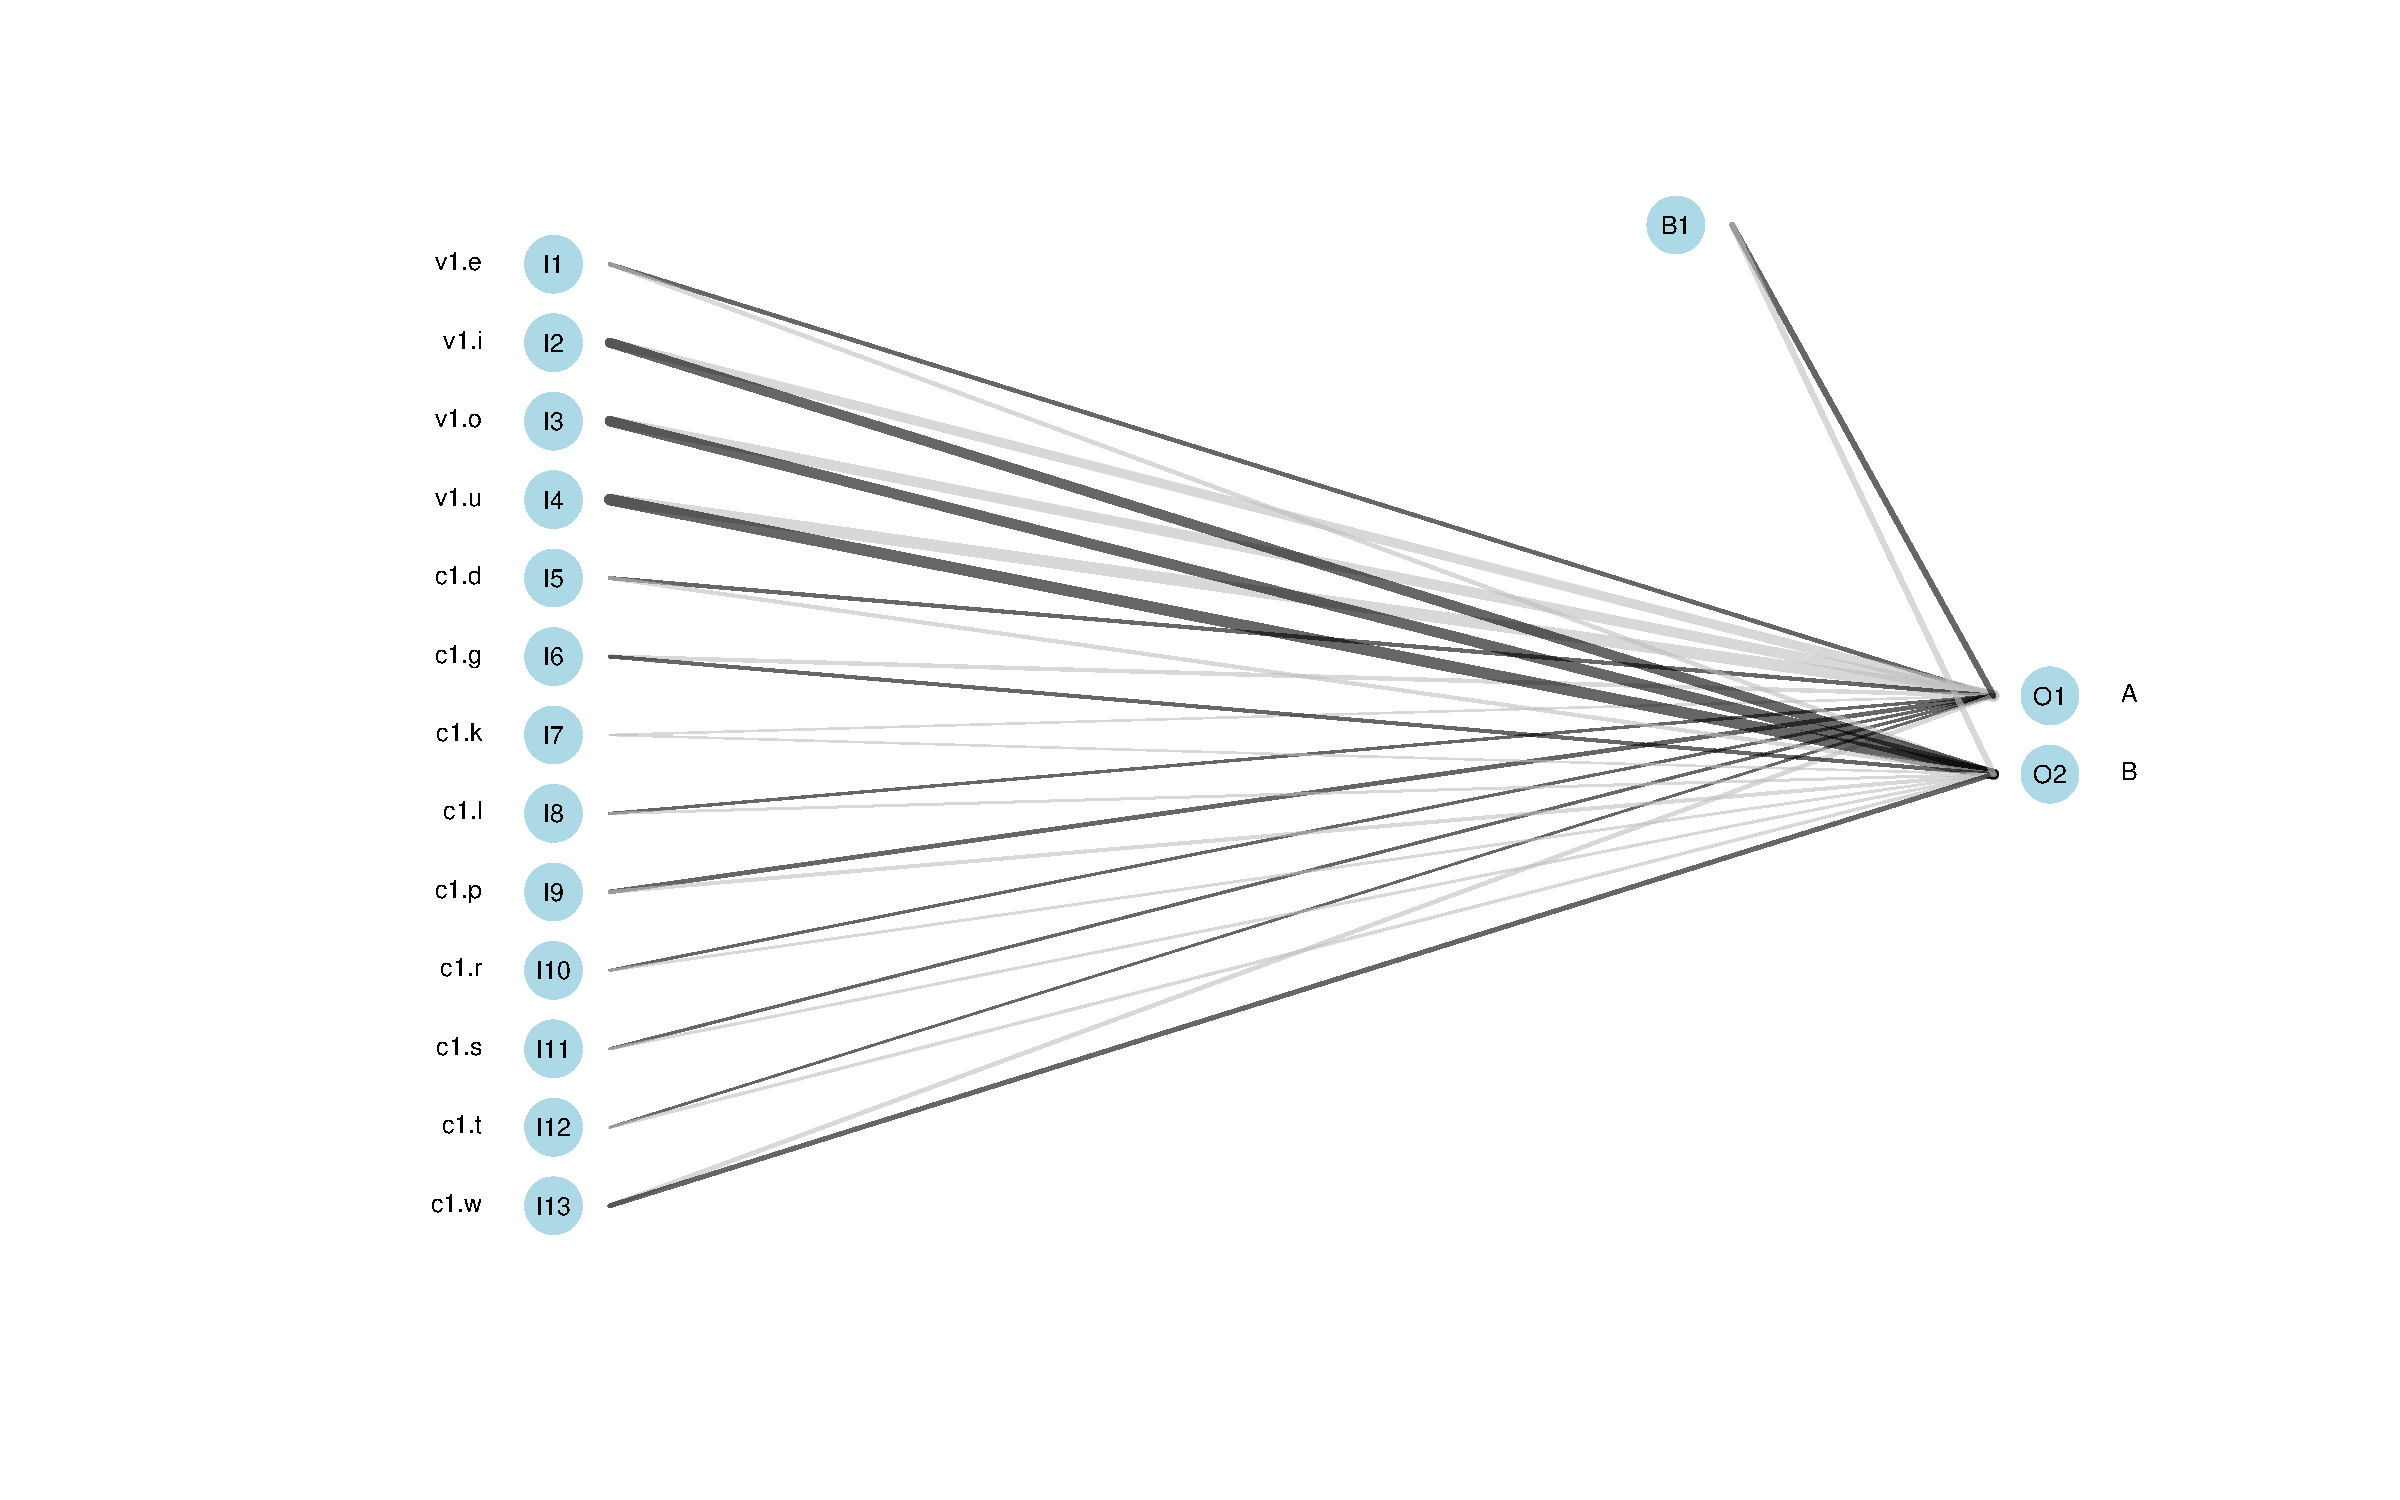
\includegraphics[scale=0.5]{./figures/fake/model2.pdf}
  \caption{Representation of Model 2.}\label{fig:model2}
\end{sidewaysfigure}

\begin{table}[!htpb]
  \centering
  \begin{tabular}{lllll}
    \lsptoprule
       & weight & predictor & response & variable \\
    \midrule
    1  & 7.43   & a-c       & A        & baseline \\
    2  & 11.87  & e         & A        & v1       \\
    3  & -21.81 & i         & A        & v1       \\
    4  & -24.18 & o         & A        & v1       \\
    5  & -34.05 & u         & A        & v1       \\
    6  & 5.77   & d         & A        & c1       \\
    7  & -6.66  & g         & A        & c1       \\
    8  & 0.34   & k         & A        & c1       \\
    9  & 6.80   & l         & A        & c1       \\
    10 & 5.68   & p         & A        & c1       \\
    11 & -2.33  & r         & A        & c1       \\
    12 & 5.48   & s         & A        & c1       \\
    13 & -3.36  & t         & A        & c1       \\
    14 & -8.98  & w         & A        & c1       \\
    15 & -8.19  & a-c       & B        & baseline \\
    16 & -12.23 & e         & B        & v1       \\
    17 & 22.95  & i         & B        & v1       \\
    18 & 25.17  & o         & B        & v1       \\
    19 & 34.15  & u         & B        & v1       \\
    20 & -5.20  & d         & B        & v1       \\
    21 & 7.28   & g         & B        & c1       \\
    22 & 0.09   & k         & B        & c1       \\
    23 & -6.61  & l         & B        & c1       \\
    24 & -5.82  & p         & B        & c1       \\
    25 & 2.02   & r         & B        & c1       \\
    26 & -6.57  & s         & B        & c1       \\
    27 & 2.48   & t         & B        & c1       \\
    28 & 9.22   & w         & B        & c1       \\
    \lspbottomrule
  \end{tabular}\caption{Weight table for Model 2.}\label{tab:model2-weights}
\end{table}

In \tabref{tab:preds-model2} we see now the results of the predictions. This time the model only made one mistake: \textit{egrr}. The reason why \textit{grip} is correctly classified this time is that the model finds it similar enough to \textit{liz}, \textit{lip} and \textit{gin}, because it now knows what its vowel is. Trying to reconstruct the evaluation of \textit{egrr} is instructive. For obtaining the weight for \textbf{A} we add to the baseline (7.43) the weight for \texttt{c1}=\textit{g} (-6.66) and \texttt{v1}=\textit{e} (11.87), which gives us 12.64, and we do the same for \textbf{B} (-8.19-12.23+7.28) and we get -13.14. This clearly makes \textbf{A} win, but the node for \texttt{c1} was pulling, in both cases, for \textbf{B}. This means that even though the model made the wrong choice, it did see a similarity between \textit{egrr} and other \textbf{B} items (namely having \textit{g} as its first consonant). This can be seen in the probabilities in \tabref{tab:preds-model2}. Of those items classified as \textbf{A}, \textit{eggr} had the highest (even if small) probability of belonging to class \textbf{B}. I will use this aspect of the analogical models in the next chapters to measure similarity between classes.

\begin{table}[!htpb]
  \centering
  \begin{tabular}{llllll}
    \lsptoprule
      & Predicted & Probability A & Probability B & Observed & Word \\
    \midrule
    1 & A         & 9.99e-01      & 3.25e-07      & A        & lama \\
    2 & A         & 9.99e-01      & 3.25e-07      & A        & lara \\
    3 & A         & 9.99e-01      & 5.20e-07      & A        & kar  \\
    4 & A         & 9.99e-01      & 3.18e-06      & B        & egrr \\
    5 & B         & 5.14e-05      & 9.99e-01      & B        & liz  \\
    6 & B         & 1.83e-04      & 9.99e-01      & B        & oppe \\
    7 & B         & 5.55e-09      & 1.00e+00      & B        & grip \\
    \lspbottomrule
  \end{tabular}
  \caption{Predictions Model 2, including the probabilities for class \textbf{A} and \textbf{B}.}\label{tab:preds-model2}
\end{table}

The corresponding confusion matrix and statistics for Model 2 are given in \tabref{tab:model2-conf} and \tabref{tab:stats-model2}, respectively.

\begin{table}[!htpb]
  \centering
  \begin{tabular}{rrrr}
    \lsptoprule
               & \multicolumn{3}{c}{Reference} \\
    \midrule
    Prediction & A  & B                        \\
    A          & 3  & 1                        \\
    B          & 0  & 3                        \\
    \lspbottomrule
  \end{tabular}
  \caption{Confusion matrix for Model 2.}\label{tab:model2-conf}
\end{table}

\begin{table}[!htpb]
  \centering
  \begin{tabular}{llrr}
    \lsptoprule
    \multicolumn{2}{c}{Overall statistics:} \\

    \midrule
    Accuracy            & 0.8571            \\
    95\% CI             & (0.4213, 0.9664)  \\
    No Information Rate & 0.5714            \\
    Kappa               & 0.72              \\
    \lspbottomrule
  \end{tabular}
  \caption{Overall statistics for Model 2.}\label{tab:stats-model2}
\end{table}

One final important point is that we see how the CI and the Kappa are partially independent of each other. In Model 2, we obtained a Kappa of 0.72, which is considerably higher than what we would get in a random model, but because this metric is not sensitive to sample size, it fails to take into account the fact that there are only seven observations. The CI information, on the other hand, does take this into account and rightly tells us that we cannot draw any conclusion from this tiny dataset. I will use both metrics together when evaluating models.

The models in the following chapters are too large and complex to either plot, or explore by hand. For this reason I will only make use of confusion matrices and accuracy scores to evaluate them, but in principle it would be possible for someone to inspect any of the analogical models presented here.

\section{Measuring variable importance}

\is{Variable importance}

An issue with neural networks is the fact that it is relatively difficult to interpret the exact importance that the different factors have on the overall model. Unlike linear or logistic regression, we cannot directly explore the coefficients. However, in some cases, it is important to understand which factor plays a more or less important role predicting some dataset. To address this question we can make use of additive and subtractive modelling. The idea is very simple. For subtractive modelling we start with the complete model (with all predictors), and we compare its accuracy and kappa scores to models leaving one predictor out. This technique allows us to compare the relative importance of each individual predictor in the context of the complete model, each individual predictor is. The additive variant of this idea consists of starting with a null model without predictors, and one by one, adding the original predictors back and comparing at each step the accuracy and kappa scores.

\section{Clustering and distances between classes}

\is{Clustering}
\is{Class distance}

The second important method I will use throughout this book is that of clustering and measuring class similarity. Imagine the new made up set of stems whose inflectional class we want to predict as shown in \REF{inf-class-2}:

\begin{exe}
    \ex \label{inf-class-2}
    \begin{xlist}
        \ex A: \textit{lama}, \textit{lara}, \textit{lado}, \textit{laso}, \textit{tama}, \textit{ga}, \textit{gal}, \textit{tar}, \textit{tsar}, \textit{tek}, \textit{tess}
        \ex B: \textit{egrr}, \textit{liz}, \textit{lo}, \textit{loi}, \textit{le}, \textit{lep}, \textit{loop}, \textit{olpe}, \textit{toi}, \textit{olor}, \textit{gen}, \textit{grap}, \textit{tak}
        \ex C: \textit{yrro}, \textit{yrto}, \textit{yro}, \textit{undo}, \textit{ujo}, \textit{jyr}, \textit{juk}, \textit{juz}, \textit{ryk}
    \end{xlist}
\end{exe}

In this new example we have three classes (\textbf{A}, \textbf{B} and \textbf{C}) which are easily described in terms of their first vowels and consonants. Words in \textbf{A} have an \textit{a}, or an \textit{e} preceded by a \textit{t}, \textit{s} or \textit{g}. Words in \textbf{B} have an \textit{o}, \textit{i}, \textit{a}, or an \textit{e} not preceded by a \textit{t} (except for \textit{tak}). Words in \textbf{C} have a \textit{y} or \textit{u}, usually with an \textit{r} or \textit{j}. Additionally, we can observe that there is a much greater similarity between \textbf{A} and \textbf{B}, than \textbf{C} to the other two. \textbf{A} and \textbf{B} can appear with an \textit{l} or \textit{e}, and to a lesser degree \textit{t} or \textit{g}, while \textbf{C} does not.

We can fit a new model using again the predictors \texttt{c1} and \texttt{v1} to this new dataset (Model 3), and because the system is much more regular now, it should predict perfectly the class of an item. What we really want to achieve now is measuring the similarity between the three classes based on the analogical model. This can be done in different ways. In a model with few classes and lots of errors between the classes, we could look at the degree of confusion between any two classes and set classes with more confusion as more similar. In models with many classes this is less practical because class size is Zipf distributed \autocite{Blevins.2016}, which means that many classes will have very few members. In highly accurate models with very few errors, the measured similarity for small classes will be much less reliable. An alternative I will use in this situation is to directly use the probabilities predicted by the model.

The probabilities for Model 3 can be seen in \tabref{tab:probabilities-model3}\footnote{For the purposes of this example I am not splitting the dataset into training and testing sets. For the actual case studies the probabilities used come from the same cross-validation process.}. In this table, each line shows the probabilities a stem has of belonging to either of the three classes. So, for \textit{lama}, the probabilities are 0.8496 for class \textbf{A}, 0.1503 for class \textbf{B}, and 6.225e-09 for class \textbf{C}. From these probabilities we can build a (negative) correlation distance matrix\footnote{When using errors instead of probabilities the process is the same, but we take the negative correlation measures for the confusion matrix instead.} and from this, a distance matrix as shown in \tabref{tab:corr-dist-model3}.

\begin{table}[!htpb]
  \centering
  \begin{tabular}{lllll}
    \toprule
       & Probability A & Probability B & Probability C & Word \\
    \midrule
    1  & 8.496e-01     & 1.503e-01     & 6.225e-09     & lama \\
    2  & 8.496e-01     & 1.503e-01     & 6.225e-09     & lara \\
    3  & 8.496e-01     & 1.503e-01     & 6.225e-09     & lado \\
    4  & 8.496e-01     & 1.503e-01     & 6.225e-09     & laso \\
    5  & 9.512e-01     & 4.873e-02     & 5.017e-12     & tama \\
    6  & 5.987e-01     & 4.012e-01     & 3.328e-11     & ga   \\
    7  & 5.987e-01     & 4.012e-01     & 3.328e-11     & gal  \\
    8  & 9.512e-01     & 4.873e-02     & 5.017e-12     & tar  \\
    9  & 9.512e-01     & 4.873e-02     & 5.017e-12     & tsar \\
    10 & 5.974e-01     & 4.025e-01     & 1.745e-11     & tek  \\
    11 & 5.974e-01     & 4.025e-01     & 1.745e-11     & tess \\
    12 & 1.018e-01     & 8.981e-01     & 3.138e-11     & egrr \\
    13 & 5.833e-23     & 1.000e+00     & 1.999e-19     & liz  \\
    14 & 2.353e-17     & 1.000e+00     & 4.455e-15     & lo   \\
    15 & 2.353e-17     & 1.000e+00     & 4.455e-15     & loi  \\
    16 & 3.006e-01     & 6.993e-01     & 1.220e-08     & le   \\
    17 & 3.006e-01     & 6.993e-01     & 1.220e-08     & lep  \\
    18 & 2.353e-17     & 1.000e+00     & 4.455e-15     & loop \\
    19 & 2.353e-17     & 1.000e+00     & 4.455e-15     & olpe \\
    20 & 8.127e-17     & 1.000e+00     & 1.107e-17     & toi  \\
    21 & 2.353e-17     & 1.000e+00     & 4.455e-15     & olor \\
    22 & 1.018e-01     & 8.981e-01     & 3.138e-11     & gen  \\
    23 & 5.987e-01     & 4.012e-01     & 3.328e-11     & grap \\
    24 & 9.512e-01     & 4.873e-02     & 5.017e-12     & tak  \\
    25 & 6.060e-11     & 7.044e-14     & 1.000e+00     & yrro \\
    26 & 6.060e-11     & 7.044e-14     & 1.000e+00     & yrto \\
    27 & 6.060e-11     & 7.044e-14     & 1.000e+00     & yro  \\
    28 & 1.308e-11     & 1.154e-13     & 1.000e+00     & undo \\
    29 & 5.052e-12     & 7.686e-15     & 1.000e+00     & ujo  \\
    30 & 1.162e-09     & 1.756e-12     & 1.000e+00     & jyr  \\
    31 & 5.052e-12     & 7.686e-15     & 1.000e+00     & juk  \\
    32 & 5.052e-12     & 7.686e-15     & 1.000e+00     & juz  \\
    33 & 6.060e-11     & 7.044e-14     & 1.000e+00     & ryk  \\
    \bottomrule
  \end{tabular}
  \caption{Predicted probabilities for Model 3.}\label{tab:probabilities-model3}
\end{table}

\begin{table}[!htpb]
  \centering
  \begin{tabular}{llll}
    \toprule
    \multicolumn{4}{c}{Correlation matrix} \\
    \midrule
      & A      & B      & C                \\
    \midrule
    A & 0.000  & -1.359 & -1.533           \\
    B & -1.359 & 0.000  & -1.598           \\
    C & -1.533 & -1.597 & 0.000            \\
    \midrule
    \multicolumn{4}{c}{As distances}       \\
      & A      & B                         \\
    \midrule
    B & 0.359  &                           \\
    C & 0.533  & 0.598                     \\
    \bottomrule
  \end{tabular}
  \caption{Correlation distances for Model 3.}\label{tab:corr-dist-model3}
\end{table}

From the distance matrix we can see that \textbf{A} is closest (has the smaller distance) to \textbf{B}, and that the greater distance is between \textbf{B} and \textbf{C}. Using the distance matrix we can then build a dendrogram using hierarchical clustering\footnote{For the clustering I use the Ward's linkage method. Although Ward's method \autocite{Murtagh.2014} is designed to be applied to Euclidean distances, some recent studies have shown it performs formidably with other distance metrics \autocites{Meyniel.2010, Strauss.2017}.} \autocite{Rokach.2005} as in \figref{fig:dendro-model3}. Similarly, we can compress the information given in the correlation matrix from three to two dimensions using multidimensional scaling (MDS) \autocite{Borg.2005, Cysouw.2007c}. Informally, MDS is a way of visualizing highly dimensional data in a two-dimensional plot. It tries to preserve as much of the original distance between two objects as possible. There is an inherent data loss when using MDS, which means the plots are an approximation, and there is dimensional data in the original distance matrix being lost. Using this two-dimensional representation of the data we can plot the categories on a two-dimensional plane as in \figref{fig:mds-model3}.

\begin{figure}[!htpb]
  \centering
  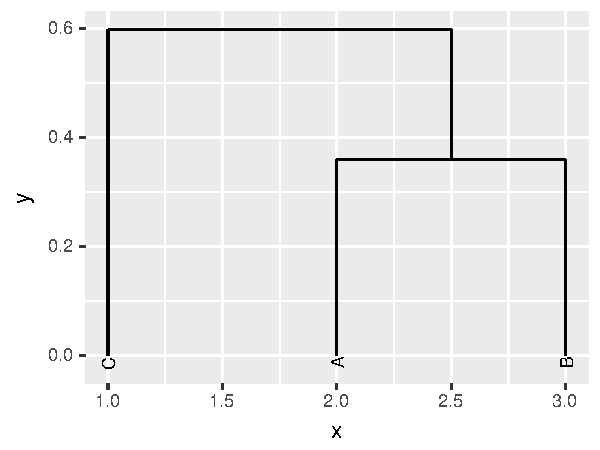
\includegraphics{./figures/fake/dendro3.pdf}
  \caption{Dendrogram based on correlation distances for Model 3.}\label{fig:dendro-model3}
\end{figure}

\begin{figure}[!htpb]
  \centering
  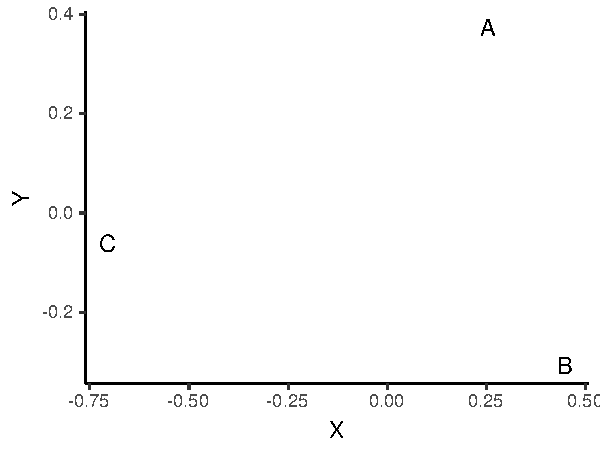
\includegraphics{./figures/fake/mds3.pdf}
  \caption{MDS based on correlation distances for Model 3.}\label{fig:mds-model3}
\end{figure}

In this case, both representations agree with the observation from before: \textbf{A} and \textbf{B} are closer to each other than to \textbf{C}. Additionally, \figref{fig:dendro-model3} shows that \textbf{A} is somewhat closer to \textbf{C} than \textbf{B} is. For simple cases with only three groups I will only make use of dendrograms, but for cases with many classes I will also use MDS.

\section{Summing up}

I have shown in this chapter that building analogical models with neural networks is not conceptually different from finding analogical relations by hand. The statistical models are, to a great extent, a notational variant of informal descriptions or schemas. They have the advantage that they require less manual work and can be easily applied to very large datasets. The clustering analysis with dendrograms and the MDS analysis for finding similar classes does not produce substantially different results from what a linguist would arrive at by inspecting the items manually. As stated before, there is no claim about the cognitive reality or psycholinguistic plausibility of the neural networks themselves. Neural networks are simply tools. The claim is that the analogical relations are present in the data, and speakers can thus make use of these relations.

In the next chapters I will use these tools to explore different analogical systems in various languages. Part II contains four chapters besides this one, each corresponding to a general topic and containing at least two case studies. Chapter \sectref{chap:gender-assignment} deals with some general gender issues in Latin and Romanian. This chapter introduces the basic claim, and shows how analogical relations that predict gender in nouns have a correlate with the hierarchy. Chapter \sectref{chap:hybrid} shows what happens in systems where simple trees are not enough and we need hybrid types in the hierarchy. This chapter deals with the topic of overabundance and affix competition in Russian and Croatian. Chapter \sectref{chap:structural} explores the claim that we need structural information in the analogical models. I present examples from prefixing languages (Swahili and Otomí de la Sierra), where the analogical process takes place on the first segments of the items, and Hausa, were the analogical specification requires more structure than for other languages. Chapter \sectref{chap:complex} presents three cases of complex inflectional systems: Spanish verb classes and Kasem number classes. This chapter provides the strongest evidence for the interaction between type hierarchies and analogical processes. Finally, Chapter \sectref{chap:conclusion} sums up the results and their implications for both usage-based and formal linguistics.

%%%%%%%%%%%%%%%%%%%%%%%%%%%%%%%%%%%%%%%%
%%%%%%%%%%%%%%%%%%%%%%%%%%%%%%%%%%%%%%%%
%%%%%%%%%%%%%%%%%%%%%%%%%%%%%%%%%%%%%%%%

%%% Local Variables:
%%% mode: latex
%%% TeX-master: "../main"
%%% End:
